\documentclass[t,pdf]{beamer}
\mode<presentation>{}


\usecolortheme[RGB={196, 30, 58}]{structure}

\usepackage{color}
\usepackage{animate}
\usepackage{tikz}
\usetikzlibrary{shadings,shadows}
\usetikzlibrary{shapes, arrows}
\usetikzlibrary{decorations.pathreplacing,angles,quotes}
\usetikzlibrary{calc}
\usetikzlibrary{positioning}
\usepackage{pgfplots}
\usepackage{booktabs}
\usepackage{alltt}
\usepackage{bussproofs}

\newenvironment{ccode}{\begin{alltt}\footnotesize}{\end{alltt}}

\usepackage{booktabs,colortbl}

\usepackage{hyperref}
%% Colored hyperlink 
\newcommand{\cref}[2]{\href{#1}{\color{blue}#2}}
%% Colored hyperlink showing link in TT font
% \newcommand{\chref}[1]{\href{#1}{\small\tt \color{blue}#1}}
\newcommand{\hcref}[1]{\cref{#1}{\small\tt #1}}


\newcommand{\ground}{blue}

\newcommand{\ft}[1]{\frametitle{#1}}
\newcommand{\ig}[2]{\includegraphics[#1]{#2}}

\definecolor{xred}{rgb}{0.77, 0.12, 0.23}
\definecolor{xgreen}{rgb}{0.3, 0.6, 0}
\definecolor{xblue}{rgb}{0., 0.25, 1}
\tikzstyle{grayfill} = [fill=fillcolor!70, draw=drawcolor, thick]
\tikzstyle{whitefill} = [fill=white, draw=drawcolor, thick] 
\definecolor{fillcolor}{rgb}{0.5, 0.5, 0.5} 
\definecolor{drawcolor}{rgb}{0, 0, 0} 

\newcommand{\hdomino}[2]{\draw [draw=black, fill=black, rounded corners=2pt] (#1+0.1,#2+0.1) rectangle (#1+1.9,#2+0.9);}
\newcommand{\vdomino}[2]{\draw [draw=black, fill=black, rounded corners=2pt] (#1+0.1,#2+0.1) rectangle (#1+0.9,#2+1.9);}

\newcommand{\hdomina}[2]{\draw [draw=black, fill=black, rounded corners=2pt] (#1+0.1,#2+0.1) rectangle (#1+1.9,#2+0.9);
                                              \draw [very thick, draw=xgreen] (#1,#2) rectangle (#1+2,#2+1);
                                              \draw [very thick, draw=structure] (#1+1,#2) -- (#1+1,#2+1);}
\newcommand{\hdominah}[2]{\draw [draw=black, fill=black, rounded corners=2pt] (#1+0.1,#2+0.1) rectangle (#1+1.9,#2+0.9);
%                                              \draw [very thick, draw=xgreen] (#1,#2) rectangle (#1+2,#2+1);
                                              \draw [very thick, draw=structure] (#1+1,#2) -- (#1+1,#2+1);}
\newcommand{\vdomina}[2]{\draw [draw=black, fill=black, rounded corners=2pt] (#1+0.1,#2+0.1) rectangle (#1+0.9,#2+1.9);
                                              \draw [very thick, draw=xgreen] (#1,#2) rectangle (#1+1,#2+2);
                                              \draw [very thick, draw=structure] (#1,#2+1) -- (#1+1,#2+1);}

\newcommand\setrow[9]{
  \setcounter{col}{1}
  \foreach \n in {#1, #2, #3, #4, #5, #6, #7, #8, #9} {
    \edef\x{\value{col} - 0.5}
    \edef\y{9.5 - \value{row}}
    \node[anchor=center] at (\x, \y) {\n};
    \stepcounter{col}
  }
  \stepcounter{row}
}

\font\dominos=domino
\def\die#1{{\dominos#1}}

\newcommand\PlaceDot[2]{\fill[white] ([shift={(#1,#2)}]0,0) circle [radius=0.08];}

\newcommand\domino[1]{
{
\ifcase#1\relax
\or \PlaceDot{0}{0}
\or \PlaceDot{-0.25}{0.25}\PlaceDot{0.25}{-0.25}
\or \PlaceDot{-0.25}{0.25}\PlaceDot{0}{0}\PlaceDot{0.25}{-0.25}
\or \PlaceDot{-0.25}{0.25}\PlaceDot{0.25}{0.25}\PlaceDot{-0.25}{-0.25}\PlaceDot{0.25}{-0.25}
\or \PlaceDot{-0.25}{0.25}\PlaceDot{0.25}{0.25}\PlaceDot{0}{0}\PlaceDot{0.25}{-0.25}\PlaceDot{-0.25}{-0.25}
\or \PlaceDot{-0.25}{0.25}\PlaceDot{0.25}{0.25}\PlaceDot{-0.25}{0}\PlaceDot{0.25}{0}\PlaceDot{0.25}{-0.25}\PlaceDot{-0.25}{-0.25}
\fi}
}


\title{Trustworthy Boolean Reasoning \\ 1A: (Un)Satisfiability}
%\subtitle{}
\author{Randal E. Bryant}


\institute{
\includegraphics[height=50pt]{figs/CMU_Logo}}

\date{\textcolor{black}{\today}}

\setbeamertemplate{footline}
{
	\leavevmode%
	\hbox{%
	\begin{beamercolorbox}[wd=0.35\paperwidth,ht=2.25ex,dp=1ex,center]{author in head/foot}%
	\tiny {Bryant: SSFT22}
			\vspace{4pt}
	\end{beamercolorbox}%
	\begin{beamercolorbox}[wd=0.45\paperwidth,ht=2.25ex,dp=1ex,center]{author in head/foot}%
	\end{beamercolorbox}%
	\begin{beamercolorbox}[wd=0.2\paperwidth,ht=2.5ex,dp=1ex,right]{date in head/foot}%
		\structure{\scriptsize \insertframenumber{} / \inserttotalframenumber\hspace*{3ex}}
		\vspace{3pt}
	\end{beamercolorbox}}%
	\vskip0pt%
}

\beamertemplatenavigationsymbolsempty

\begin{document}

\newcommand{\R}{\mathbb{R}}
\renewcommand{\P}{\mathbb{P}}
\newcommand{\E}{\mathbb{E}}
\newcommand{\Z}{\mathbb{Z}}
\newcommand{\N}{\mathbb{N}}
\newcommand{\diam}{\mbox{diam}}

\newcommand{\obar}[1]{\overline{#1}}
\newcommand{\xnot}{\obar{x}}
\newcommand{\anot}{\obar{a}}
\newcommand{\bnot}{\obar{b}}
\newcommand{\cnot}{\obar{c}}
\newcommand{\dnot}{\obar{d}}
\newcommand{\tnot}{\obar{t}}
\newcommand{\znot}{\obar{z}}

\newtheorem{conjecture}[theorem]{Conjecture}
\newtheorem{nonconj}[theorem]{(Not actually a) conjecture}


\begin{frame}
	\titlepage
\end{frame}



\frame{
  \frametitle{Important Ideas for These Lectures}
  \begin{itemize}
  \item SAT solvers are useful tools
    \begin{itemize}
    \item Many practical problems reducible to SAT
    \item Need to learn effective encoding techniques
    \end{itemize}
\medskip
  \item For many applications, formulas should be unsatisfiable
    \begin{itemize}
    \item Only trust result if program generates a checkable proof
    \item There is a well-developed proof infrastructure
    \end{itemize}

\medskip
  \item Binary Decision Diagrams (BDDs) can play important role
    \begin{itemize}
    \item In supplementing current SAT algorithms
    \item In proof generation
    \end{itemize}
  \end{itemize}


}

\begin{frame}[fragile]
  \frametitle{SAT Application: Bit-Level Program Verification}
{\large \em  \textcolor{xblue}{Are these functions equivalent?}}\\
\medskip

\begin{minipage}[t]{0.48\textwidth}
\begin{ccode}
int abs_new(int x) \verb:{:
  int m = x>>31;
  return x^m + ~m + 1;
\verb:}:

int abs_ref(int x) \verb:{:
  return x < 0 ? -x : x;
\verb:}:    
\end{ccode}
\end{minipage}
\begin{minipage}[t]{0.48\textwidth}
\begin{ccode}
\end{ccode}
\end{minipage}

\medskip
\begin{itemize}
\item Assume for {\tt int}:
  \begin{itemize}
  \item 32-bit word
  \item Two's complement representation
  \end{itemize}
\end{itemize}
\end{frame}

\begin{frame}[fragile]
  \frametitle{SAT Application: Bit-Level Program Verification}
{\large \em \textcolor{xblue}{Can this program call \texttt{ERROR}?}}\\

\medskip
\begin{minipage}[t]{0.48\textwidth}
\begin{ccode}
int abs_new(int x) \verb:{:
  int m = x>>31;
  return x^m + ~m + 1;
\verb:}:

int abs_ref(int x) \verb:{:
  return x < 0 ? -x : x;
\verb:}:    
\end{ccode}
\end{minipage}
\begin{minipage}[t]{0.48\textwidth}
\begin{ccode}
int main() \verb:{:
  /* Value of t arbitrary */
  int t = random();
  int vn = abs_new(t);
  int vr = abs_ref(t);
  int err = (vn != vr);
  if (err != 0)
    ERROR();
\verb:}:
\end{ccode}
\end{minipage}

\medskip
\begin{itemize}
\item Assume for {\tt int}:
  \begin{itemize}
  \item 32-bit word
  \item Two's complement representation
  \end{itemize}
\end{itemize}
\end{frame}


\begin{frame}
  \frametitle{Application: Bit-Level Program Verification}
      {\bf C Bounded Model Checker (CBMC)}
      \begin{itemize}
      \item Clarke, Kroening, Lerda  TACAS 2004
      \end{itemize}
\medskip
      {\bf Reduces Program Verification to SAT}
      \begin{itemize}
      \item Unroll loops by bounded amount
      \item Represent all data types as bit vectors (``Bit-Blasting'')
      \item Encode output of {\tt random} as vector of Boolean variables.
      \item Encode arithmetic and logical operations at Boolean level
      \item Formula satisfied if {\tt err} can be nonzero
        \begin{itemize}
          \item Unsatisfiable when no error can occur
        \end{itemize}
      \end{itemize}
      \medskip
      {\bf Widely Used in Industry}
      \begin{itemize}
      \item Accurately models low-level program behavior
      \item Good for short, but tricky programs
      \end{itemize}

\end{frame}


\begin{frame}
\frametitle{SAT Application: Coloring Pythagorean Triples}

{\bf Pythagorean Triple (P-Triple)}
\begin{itemize}
\item Positive integers $a$, $b$, $c$ such that $a^2 + b^2 = c^2$
\item E.g., $a=3$, $b=4$, $c=5$.
\end{itemize}

{\bf Two-Coloring}
\begin{itemize}
\item For integers $i \in \{1, 2, \ldots, n\}$, assign $C_i \in \{\textsf{red}, \textsf{blue}\}$
\item For every P-Triple $a, b, c$, Cannot have $C_a = C_b = C_c$.
\end{itemize}

\only<1>{
{\bf Question}
\begin{itemize}
\item What is the maximum $n$ for which a two-coloring exists?
\end{itemize}
}

\only<2>{
{\bf SAT Encoding ${\it PTC}(n)$}
\begin{itemize}
  \item $n$ Boolean variables
  \item Variable $x_a = 1$ if $a$ colored red, $= 0$ if colored blue
  \item Clauses for each P-Triple $a, b, c$:\\
    \begin{tabular}{ll}
       $x_a \lor x_b \lor x_c$ & At least one colored red \\
       $\xnot_a \lor \xnot_b \lor \xnot_c$ & At least one colored blue \\
    \end{tabular}
\end{itemize}
}
\end{frame}


\begin{frame}
\frametitle{SAT Application: Coloring Pythagorean Triples, $n=7824$}

\begin{center}
  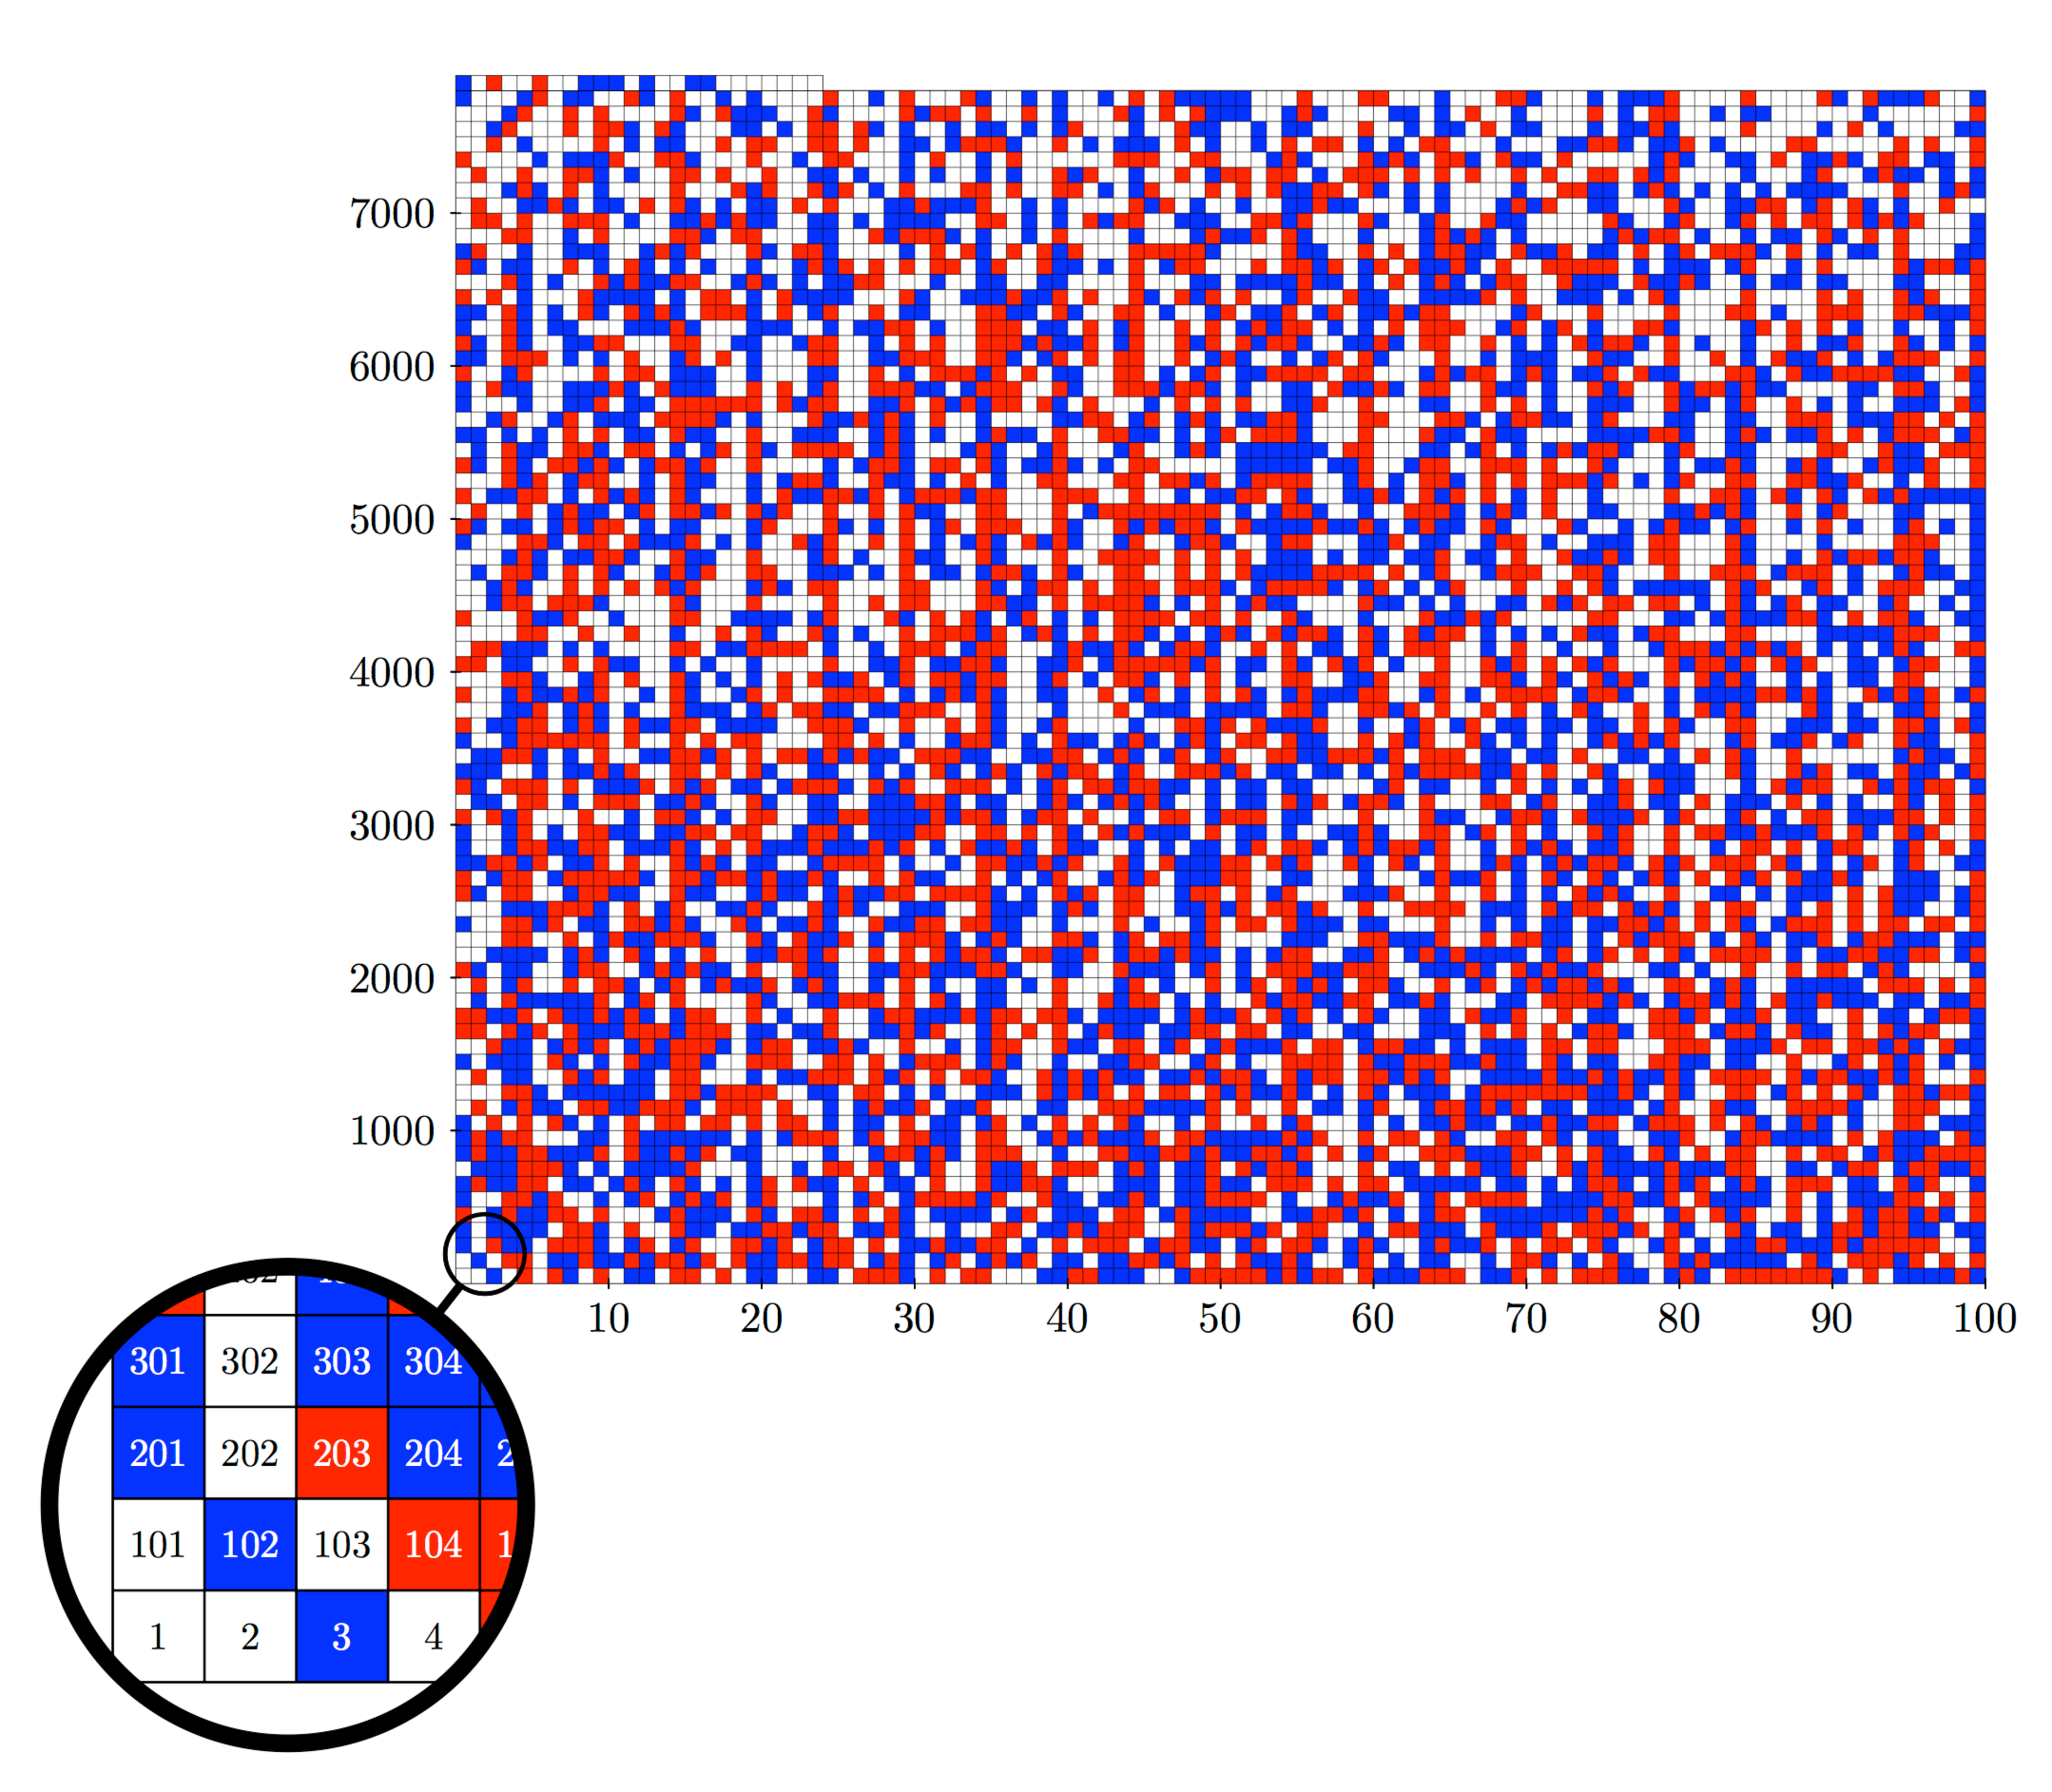
\includegraphics[height=3in]{figs/triple7824}
\end{center}

\end{frame}

\begin{frame}
\frametitle{SAT Application: Coloring Pythagorean Triples, $n\geq 7825$}

{\bf Formula ${\it PTN}(7825)$ unsatisfiable}
\begin{itemize}
\item Heule, Kullmann, Marek, SAT 2016

\medskip

\item Partitioned into $10^6$ subproblems
  \begin{itemize}
    \item By enumerating assignments for some of the variables
  \end{itemize}

\medskip

  
\item Ran on 800-core supercomputer for two days

\medskip

\item Generated proof of unsatisfiability
  \begin{itemize}
  \item 200 Terabytes total
  \item Validated with proof checker
  \item A very long and very tedious proof!
  \end{itemize}
\end{itemize}

\end{frame}

\frame{
\frametitle{Boolean Satisfiability Solvers}


\begin{tikzpicture}


\node[text width=1.5cm] (F) at (0,0) {Boolean formula};
\node[regular polygon,regular polygon sides=4, minimum size=3.5cm, draw,fill=structure, rounded corners] (S) at (3.5,0) {};
\node[white] at (3.5,0.5) {\huge \bf SAT};
\node[white] at (3.5,-0.5) {\huge \bf solver};
\draw[line width=3pt, -latex] (F) -- (S);
\node[white] at (10,3.75) {~};

\only<2->{
\node[text width=1.5cm] (sat) at (8,0.75) {\large \bf solution};
\node (topl) at (4.75,0.75) {~};
\draw[line width=2pt, -latex] (topl) -- (sat);
\node  at (6,1.25) {{\it satisfiable}};}


\only<4->{
\node[text width=1.5cm] (unsat) at (8,-0.75) {\large \bf ?};
\node  at (6,-0.25) {{\it unsatisfiable}};
\node (botl) at (4.75,-0.75) {~};
\draw[line width=2pt, -latex] (botl) --(unsat);}

\only<3->{
\node[rectangle, minimum height=1.5cm,minimum width=3cm, draw,fill=xgreen, rounded corners] (check) at (8.5,3) {};
\node[white] at (8.5,3.25) {\large \bf Solution};
\node[white] at (8.5,2.75) {\large \bf Checker};

\draw[line width=3pt, -latex] (F) edge [bend left=20] (check.west);
\draw[line width=2pt, -latex] (sat.north) -- (check.south);}


\end{tikzpicture}

\bigskip

\begin{minipage}{.40\textwidth}
{\bf SAT Solvers Useful}
\begin{itemize}
\item Optimization
\item Formal verification
\item Mathematical proofs
\end{itemize}
\end{minipage}
\begin{minipage}{.58\textwidth}
\only<5->{
{\bf Can We Trust Them?}
\begin{itemize}
\item No!
\item Complex software
\item e.g., KISSAT: 35K lines of code
\end{itemize}}
\end{minipage}



}


\frame{
\frametitle{Proof Generating Solvers}

\begin{tikzpicture}


\node[text width=1.5cm] (F) at (0,0) {Boolean formula};

\node[regular polygon,regular polygon sides=4, minimum size=3.5cm, draw,fill=structure, rounded corners] (S) at (3.5,0) {};
\node[white] at (3.5,0.5) {\huge \bf SAT};
\node[white] at (3.5,-0.5) {\huge \bf solver};
\node[white] at (10,3.75) {~};
\draw[line width=3pt, -latex] (F) --( S);

\only<2->{
\node[text width=1.5cm] (unsat) at (8,-0.75) {\large \bf unsatisfiability proof};
\node  at (6,-0.25) {{\it unsatisfiable}};
\node (botl) at (4.75,-0.75) {~};
\draw[line width=2pt, -latex] (botl) --(unsat);}

\only<3->{
\node[rectangle, minimum height=1.5cm,minimum width=3cm, draw,fill=xgreen, rounded corners] (check) at (8.5,3) {};
\node[white] at (8.5,3.25) {\large \bf Proof};
\node[white] at (8.5,2.75) {\large \bf Checker};

\draw[line width=3pt, -latex] (F) edge [bend left=20] (check.west);
\draw[line width=2pt, -latex] (unsat.north) -- (check.south);}

\end{tikzpicture}

\bigskip
\bigskip

\pause
\pause
\pause

\begin{minipage}{.49\textwidth}
{\bf Unsatisfiability Proof}
\begin{itemize}
\item Step-by-step proof in\\some logical framework
\end{itemize}
\end{minipage}
\begin{minipage}{.49\textwidth}
{\bf Proof Checker}
\begin{itemize}
\item Simple program
\item May be formally verified
\end{itemize}
\end{minipage}

} %% FRAME


\frame{
  \frametitle{Impact of Proof Checking}

  \begin{minipage}[t]{0.43\textwidth}
    {\bf Adoption}
    \begin{itemize}
      \item Required for SAT competition entrants since 2016
    \end{itemize}
    {\bf Benefits}
    \begin{itemize}
    \item Can clearly judge competition submissions
    \item Developers have improved quality of their solvers
    \item Firm foundation for use in mathematical proofs
    \end{itemize}
  \end{minipage}
  \begin{minipage}[t]{0.03\textwidth}
    $\;$
  \end{minipage}  
  \begin{minipage}[t]{0.50\textwidth}
    \only <2->{
    {\bf Unintended Consequences}
    \begin{itemize}
    \item Narrowed focus to single SAT algorithm
      \begin{itemize}
      \item Conflict-Driven Clause Learning (CDCL)
      \item Search for solution, but learn conflicts
      \end{itemize}
    \item Other powerful solution methods have languished.
    \end{itemize}
    }
    \only <3>{
    {\bf Long-Term Goals}
    \begin{itemize}
    \item Enable proof generation for other SAT algorithms
    \item Develop checkable proof infrastructure for other domains
    \end{itemize}
    }
  \end{minipage}
}


\frame{
\frametitle{Conjunctive Normal Form (CNF) Formulas}

{\bf Variables}
\begin{itemize}
\item Input: $X = \{x_1, x_2, \ldots, x_n\}$
\item Informally: $a, b, c, \ldots$
\end{itemize}

{\bf Literals}
\begin{itemize}
\item Variable $x$
\item Complemented variable $\xnot$.
\end{itemize}

{\bf Clauses}
\begin{itemize}
\item $C = \{l_1, l_2, \ldots, l_k\}$~~~~~Set of literals
\item $\anot \lor b \lor \cnot$
\item $\bot = \emptyset$~~~~~~~~~~~~~~~~~ Empty clause (False)
\end{itemize}

{\bf Formula}
\begin{itemize}
\item $\phi = \{C_1, C_2, \ldots, C_m\}$
\item Conjunction of clauses
\end{itemize}
}

\frame{
\frametitle{Clausal Thinking}

{\bf Useful tricks when writing CNF}

\begin{center}
  \renewcommand{\arraystretch}{1.2}
  \begin{tabular}{cc}
    \toprule
    \makebox[2in]{Boolean Formula} & \makebox[2in]{CNF} \\
    \midrule
    $a \land b \rightarrow c$ & $\anot \lor \bnot \lor c$ \\
    $a \rightarrow b \lor c$ & $\anot \lor b \lor c$ \\
    $(a \lor b) \rightarrow c$ & $(\anot \lor c) \land (\bnot \lor c)$ \\
    $a \rightarrow (b \land c)$ & $(\anot \lor c) \land (\anot \lor c)$ \\
    \midrule
    ${\it AtLeastOne}(a, b, c)$ & $a \lor b \lor c$ \\
    ${\it AtMostOne}(a, b, c)$ & $(\anot \lor \bnot) \land (\anot \lor \cnot) \land (\bnot \lor \cnot)$ \\
    \bottomrule

  \end{tabular}
\end{center}


}

\frame{
\frametitle{Clausal Thinking: Parity Encodings}

\begin{center}
  \renewcommand{\arraystretch}{1.2}
  \begin{tabular}{cc}
    \toprule
    \makebox[2in]{Boolean Formula} & \makebox[2in]{CNF} \\
    \midrule
    ${\it OddParity}(a, b, c)$ &
    $\begin{array}{ll}
      (\anot \lor \bnot \lor c) & \land\\
      (\anot \lor b \lor \cnot) & \land\\
      (a \lor \bnot \lor \cnot) & \land\\
      (a \lor b \lor c) & \\
    \end{array}$ \\
\midrule
    ${\it EvenParity}(a, b, c)$ &
    $\begin{array}{ll}
      (\anot \lor \bnot \lor \cnot) & \land\\
      (a \lor b \lor \cnot) & \land\\
      (a \lor \bnot \lor c) & \land \\
      (\anot \lor b \lor c) & \\
    \end{array}$ \\
    \bottomrule
  \end{tabular}
\end{center}
}

\frame{
\frametitle{Clausal Thinking: Parity Encodings}

\begin{center}
  \renewcommand{\arraystretch}{1.05}
  \begin{tabular}{cc}
    \toprule
    \makebox[2in]{Boolean Formula} & \makebox[2in]{CNF} \\
    \midrule
    ${\it OddParity}(a, b, c)$ &
    $\begin{array}{ll}
      (\anot \lor \bnot \lor c) & \land\\
      (\anot \lor b \lor \cnot) & \land\\
      (a \lor \bnot \lor \cnot) & \land\\
      (a \lor b \lor c) & \\
    \end{array}$ \\
\midrule
    ${\it OddParity}(a, b, c, d)$ &
    $\begin{array}{ll}
      (\anot \lor \bnot \lor \cnot \lor \dnot) & \land\\
      (a \lor b \lor \cnot \lor \dnot) & \land\\
      (a \lor \bnot \lor c \lor \dnot) & \land \\
      (\anot \lor b \lor c \lor \dnot) & \land\\
      (\anot \lor \bnot \lor c \lor d) & \land\\
      (\anot \lor b \lor \cnot \lor d) & \land\\
      (a \lor \bnot \lor \cnot \lor d) & \land\\
      (a \lor b \lor c \lor d) & \\
    \end{array}$ \\
    \bottomrule
  \end{tabular}
\end{center}
}

\frame{
  \frametitle{Parity Encoding with Intermediate Variables}
{\bf Task}
 \begin{itemize}
 \item Encode ${\it OddParity}(x_1, x_2, \ldots, x_n)$
 \item Direct encoding requires  $2^{n-1}$ clauses
 \item All combinations with even number of negative literals
 \end{itemize}

{\bf Decomposition}
     \begin{itemize}
     \item Introduce new variable $z$
     \item Directly encode ${\it EvenParity}(x_1, x_2, z)$
     \item Recursively encode ${\it OddParity}(z, x_3, x_4, \ldots, x_n)$:
       \begin{itemize}
       \item If $x_1 \oplus x_2 = 0$, then $z = 0$ and ${\it OddParity}(x_3, x_4, \ldots, x_n)$
       \item If $x_1 \oplus x_2 = 1$, then $z = 1$ and ${\it EvenParity}(x_3, x_4, \ldots, x_n)$         
       \end{itemize}
     \end{itemize}

} %% Frame

\frame{
  \frametitle{Parity Encoding with Intermediate Variables}
{\bf Decomposition}
     \begin{itemize}
     \item Directly encode ${\it EvenParity}(x_1, x_2, z)$
     \item Recursively encode ${\it OddParity}(z, x_3, x_4, \ldots, x_n)$:
     \end{itemize}
\medskip
{\bf General Form}
\begin{eqnarray*}
  z_2 &=& x_1 \oplus x_2 \\
  z_3 &=& z_2 \oplus x_3 \\
  & \cdots & \\
  z_{n-2} & = & x_{n-2} \oplus x_{n-3}\\
  z_{n-2} \oplus x_{n-1} \oplus x_n & = & 1\\
\end{eqnarray*}
\vskip -15pt
{\bf Complexity}
\begin{itemize}
\item $n-3$ additional variables
\item $4(n-2)$ clauses
\end{itemize}
} %% Frame

\frame{
\frametitle{Encoding Arbitrary Formulas / Circuits}

\begin{center}
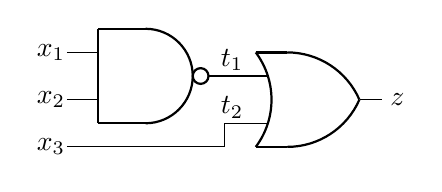
\begin{tikzpicture}[scale=0.20]
  %% NAND gate
   \draw [thick] (2,7.5) -- (5,7.5);
   \draw [thick] (2,1.5) -- (5,1.5);
   \draw [thick] (2,7.5) -- (2,1.5);
   \draw [thick] (5,1.5) arc [radius=3, start angle = -90, end angle = 90];
   \draw [thick] (8.5,4.5) circle [radius=0.5];
   %% OR gate
   \draw [thick] (12,6) -- (14,6);
   \draw [thick] (12,0) -- (14,0);
   \draw [thick] (12,6) arc [radius=5, start angle = 36.9, end angle = -36.9];
   \draw [thick] (14, 6) arc [radius=5, start angle = 90, end angle = 23.6];
   \draw [thick] (14, 0)  arc [radius=5, start angle = -90, end angle = -23.6];
   \draw (18.6,3) -- (20,3);
  %% Wire it up
  \draw (0,6) -- (2,6);
  \draw (0,3) -- (2,3);
  \draw (0,0) -- (10,0) -- (10,1.5) -- (12.8,1.5);
  \draw (9,4.5) -- (12.8,4.5);
  %% Put in labels
  \node at (-1,6) {$x_1$};
  \node at (-1,3) {$x_2$};
  \node at (-1,0) {$x_3$};
  \node at (10.5,5.5) {$t_1$};
  \node at (10.5,2.5) {$t_2$};
  \node at (21,3) {$z$};
\end{tikzpicture}
\end{center}
\renewcommand{\arraystretch}{1.1}
\begin{tabular}{lcc}
  \toprule
  \makebox[0.5in]{} & \makebox[1.75in]{Encode NAND gate} & \makebox[1.75in]{Encode OR gate} \\
  \midrule
  Formula
     & $\tnot_1 \leftrightarrow x_1 \land x_2$  
     & $z \leftrightarrow t_1 \lor t_2$  \\
  \midrule
  Clauses 
     &  $\begin{array}{l}
        t_1 \lor x_1 \\
       t_1 \lor x_2 \\
        \tnot_1 \lor \xnot_1 \lor \xnot_2\\
       \end{array}$
     &  $\begin{array}{l}
        \znot \lor t_1 \lor t_2 \\
        z \lor \tnot_1 \\
        z \lor \tnot_2 \\
       \end{array}$ \\
  \bottomrule
\end{tabular}

\medskip

    {\bf Tseitin Encoding}
    \begin{itemize}
    \item Introduce variables for intermediate values
    \item Linear complexity
    \end{itemize}


} %% FRAME

\frame{
  \frametitle{Proof Rules: Resolution}

\begin{itemize}
\item Robinson, 1965
\end{itemize}

\begin{center}
\begin{tikzpicture}
\onslide<+->{
\node at (2.5,0) {$\anot \lor b \lor \structure{x}$};
\node at (5,0) {$\structure{\xnot} \lor c \lor \dnot$};
\draw[thick] (1.5,-0.25) -- (6.2,-0.25);
\node at (3.75,-0.5) {$(\anot \lor b) \lor (c \lor \dnot)$};}
\onslide<+->{
\node at (1,1) {$(a \land \bnot) \rightarrow \structure{x}$};
\node at (6.5,1) {$\structure{x} \rightarrow (c \lor \dnot)$};}
\onslide<+->{
\node at (3.75,-1.5) {$(a \land \bnot) \rightarrow (c \lor \dnot)$};}
\end{tikzpicture}
\end{center}
\begin{itemize}
\item Generalization of implication
\item See  \hcref{https://en.wikipedia.org/wiki/Resolution\_(logic)}
\end{itemize}  


} %% FRAME

\frame{
  \frametitle{Resolution Principle Nuances}


\bigskip

{\bf OK To Have Repeated Literal}

\medskip

\begin{center}
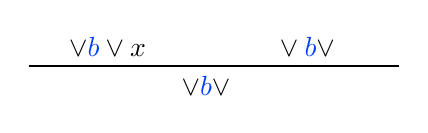
\begin{tikzpicture}
\node at (2.5,0) {$\anot \lor \textcolor{xblue}{b} \lor \structure{x}$};
\node at (5,0) {$\structure{\xnot} \lor \textcolor{xblue}{b} \lor \dnot$};
\draw[thick] (1.5,-0.25) -- (6.2,-0.25);
\node at (3.75,-0.5) {$\anot \lor \textcolor{xblue}{b} \lor \dnot$};
\end{tikzpicture}
\end{center}

\medskip

{\bf Not OK to Have Multiple Resolution Variables}

\medskip

\begin{center}
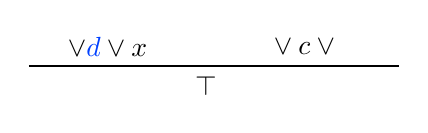
\begin{tikzpicture}
\node at (2.5,0) {$\anot \lor \textcolor{xblue}{d} \lor \structure{x}$};
\node at (5,0) {$\structure{\xnot} \lor c \lor \textcolor{xblue}{\dnot}$};
\draw[thick] (1.5,-0.25) -- (6.2,-0.25);
\node at (3.75,-0.5) {$\top$};
\end{tikzpicture}
\end{center}


} %% FRAME

\frame{
  \frametitle{Proof Rules: Subsumption}

  \bigskip
  
\begin{center}
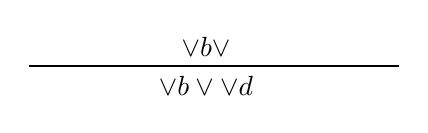
\begin{tikzpicture}
\node at (3.75,0) {$\anot \lor b \lor \cnot$};
\draw[thick] (1.5,-0.25) -- (6.2,-0.25);
\node at (3.75,-0.5) {$\anot \lor b \lor \cnot \lor \structure{d}$};
\end{tikzpicture}
\end{center}
\begin{itemize}
\item General Principle: $F \rightarrow F \lor d$
\end{itemize}  


} %% FRAME




\frame{
  \frametitle{Example Formula}

  {\bf DIMACS Format}
  \begin{itemize}
    \item Standard for all solvers
    \item Positive integers for variables
    \item Negative integers for their negations
    \item Lists terminated with {\tt 0}
  \end{itemize}  

  \begin{center}
    \begin{tabular}{cll}
      \toprule
      \makebox[0.5in]{ID} & \makebox[1.0in]{Clause} & \makebox[1.5in]{DIMACS Encoding} \\
      \midrule
      & & {\tt p cnf 4 6} \\
      1 & $\anot \lor \bnot \lor \cnot$ & {\tt -1 -2 -3 0} \\
      2 & $\anot \lor \bnot \lor c$ & {\tt -1 -2  3 0} \\
      3 & $a \lor \dnot$ & {\tt 1    -4 0} \\
      4 & $a \lor d$ & {\tt 1    4 0} \\
      5 & $b \lor \dnot$ & {\tt    2     -4 0} \\
      6 & $b \lor d$ & {\tt    2     4 0} \\
      \bottomrule
    \end{tabular}
  \end{center}
}

\frame{
  \frametitle{Example Proof}

\begin{itemize}
\item Derive empty clause $\bot$ through set of resolution steps
\end{itemize}

\begin{center}
\begin{tikzpicture}[scale = 0.8]


\node at (5.5,4.0) {$a \lor \dnot$};
\node at (7.5,4.0) {$a \lor d$};
\draw[thick] (4.5,3.5) -- (8.5,3.5);
\node at (5.0,3.0) {$a$};
\node at (8.0,3.0) {$a$};

\node at (3.0,3.0) {$\anot \lor \bnot \lor \cnot$};
\draw[thick] (2.0,2.5) -- (5.5,2.5);
\node at (4.0,2.0) {$\bnot \lor \cnot$};

\node at (10.0,3.0) {$\anot \lor \bnot \lor c$};
\draw[thick] (7.5,2.5) -- (11.0,2.5);
\node at (9.0,2.0) {$\bnot \lor c$};
\draw[thick] (3.5,1.5) -- (9.5,1.5);
\node at (6.5,1.0) {$\bnot$};

\node at (12.0,2.0) {$b \lor \dnot$};
\node at (14.0,2.0) {$b \lor d$};
\draw[thick] (11.5,1.5) -- (14.5,1.5);
\node at (13.0,1.0) {$b$};
\draw[thick] (6.0,0.5) -- (13.5,0.5);
\node at (9.750,0.0) {$\bot$};
\end{tikzpicture}

\end{center}

{\em \textcolor{xblue}{But how can a program find such a proof?}}


} %% FRAME


\end{document}

